\chapter{Integracja bazy danych ze zintegrowanym środowiskiem programistycznym}

\section{Konfiguracja SQL Server Management Studio}

Do zarządzania bazą danych wykorzystano SSMS. Rozwiązanie zostało wybrane ze względu że na co dzień mam styczność z tym środowiskiem. Jest ono łatwe w konfiguracji. Wykorzystując schemat bazy danych \ref{logowanie_etykieta} stworzono w SSMS schemat bazy danych. 
\begin{figure}[h]
    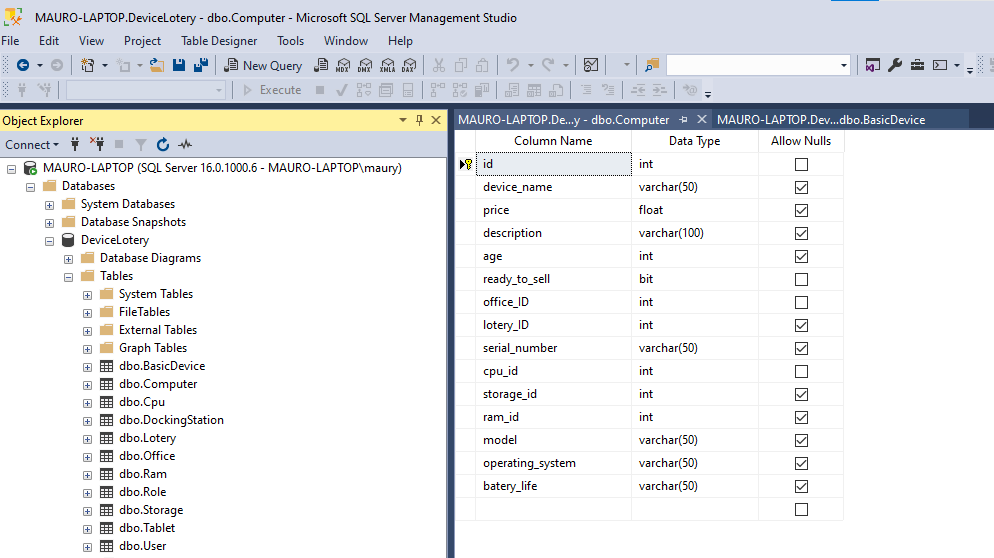
\includegraphics[scale=0.7]{rys05/ssms_tabelki.png}
    \caption{Tabelki w narzędziu SSMS}
    \label{ssms_tabelki_etykieta}
\end{figure}

\newpage
Narzędzie pozwala także na ręczne wypełnianie tabel danymi. 
\begin{figure}[h]
    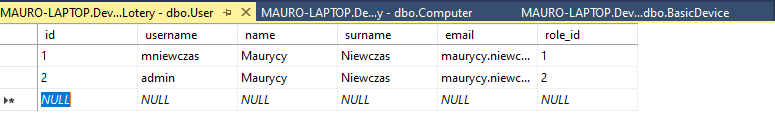
\includegraphics[scale=0.7]{rys05/dodawanie_tabel.png}
    \caption{Wypełnianie tabel danymi}
    \label{ssms_wypelnianie_tabel_etykieta}
\end{figure}

\section{Konfiguracja SQL Server Management Studio do Integracji z Intelij Idea}

Zaletą zintegrowanego środowiska programistycznego z licencją studencką {odwołanie do tabeli} jest możliwość integracji ze środowiskiem bazodanowym.
W pierwszej kolejności włączone zostało logowanie \textbf{SQL Server Autentication}

\begin{figure}[h]
    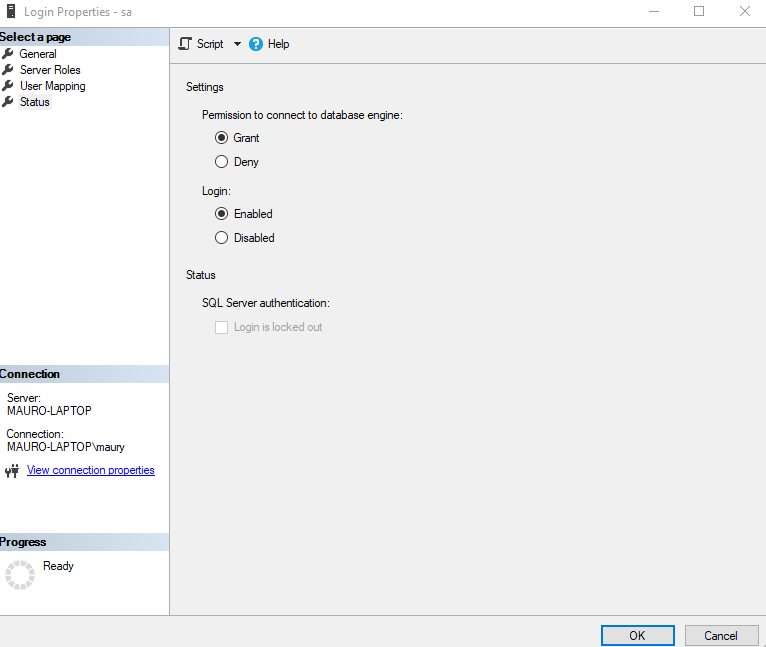
\includegraphics[scale=0.7]{rys05/login_prop.png}
    \caption{Włączenie SQL Server Autentication}
    \label{auth_etykieta}
\end{figure}

W rys. \ref{auth_etykieta} włączono SQL Server Autentication dla domyślnego uzytkownika o loginie: sa

\newpage

\begin{figure}[ht]
  \begin{minipage}[b]{0.6\linewidth}
    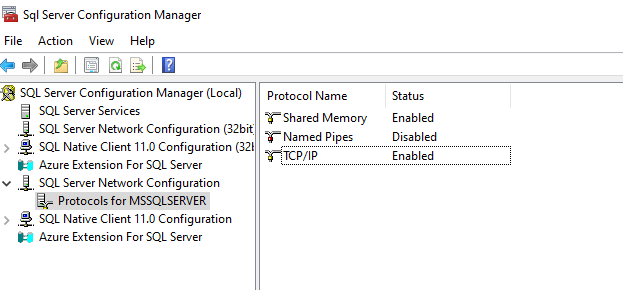
\includegraphics[width=\linewidth]{rys05/enable_tcpip.png}
    \caption{Włączenie Protokołu TCP IP dla MS SQL Server}
		\label{tcp_enable_etykieta}
  \end{minipage}
  \begin{minipage}[b]{0.5\linewidth}
    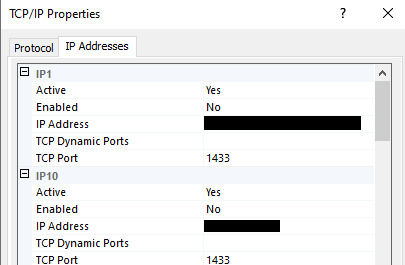
\includegraphics[width=\linewidth]{rys05/port_tcpip.png}
    \caption{Konfiguracja portu dla Protokołu TCP IP}
		\label{tcp_conf_etykieta}
  \end{minipage}
\end{figure}


Wymaganym ustawieniem do integracji SSMS z Intelij jest włączenie protokołu TCP IP dla MS SQL Server. Należało w narzędziu SQL Server Configuration Manager w protokole MS SQL Server włączyć protokół TCP IP Rys. \ref {tcp_enable_etykieta}.
Aby połączyć się z bazą danych trzeba znać port TCP IP na którym skonfigurowany jest ten protokół Rys. \ref{tcp_conf_etykieta}. Wykorzystano domyślny port zaoferowany przez narzędzie: \textbf{1433}.

\section{Konfiguracja Intelij Idea}


\begin{figure}[h]
    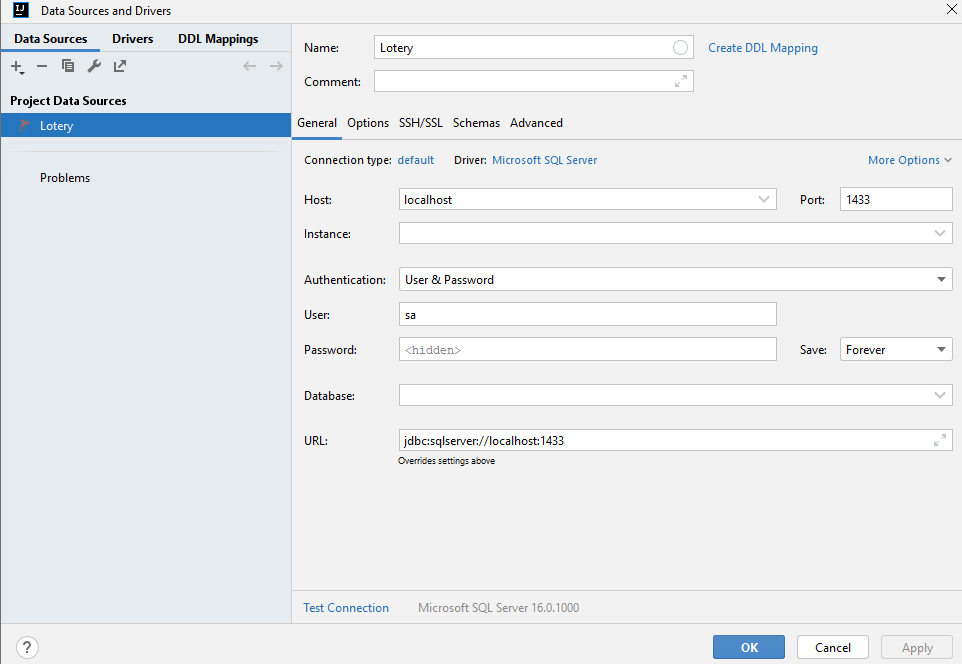
\includegraphics[scale=0.6]{rys05/intelij_config_database.png}
    \caption{Konfiguracja Intelij z Bazą danych}
    \label{intelij_db_config_etykieta}
\end{figure}

Jako port podano ten skonfigurowany w Rys. \ref{tcp_conf_etykieta}. Logowanie odbywa się na podstawie użytkownika przy użyciu SQL Server Autentication. Użytkownika skonfigurowano w SSMS w Rys. \ref{auth_etykieta} 


\newpage

\begin{figure}[h]
		\centering
    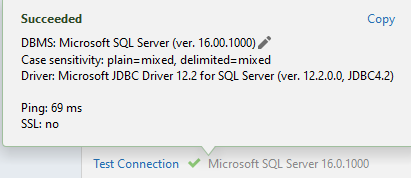
\includegraphics[scale=1.0]{rys05/test_connection.png}
    \caption{Testowanie poprawności połączenia IDE z bazą danych}
    \label{test_connection_etykieta}
\end{figure}

Po odpowiedniej konfiguracji można przetestować czy połączenie jest poprawne Rys. \ref{test_connection_etykieta}

\section{Generowanie klas w Javie przy pomocy plugina JPA Buddy}

 


\begin{figure}[h]
		\centering
    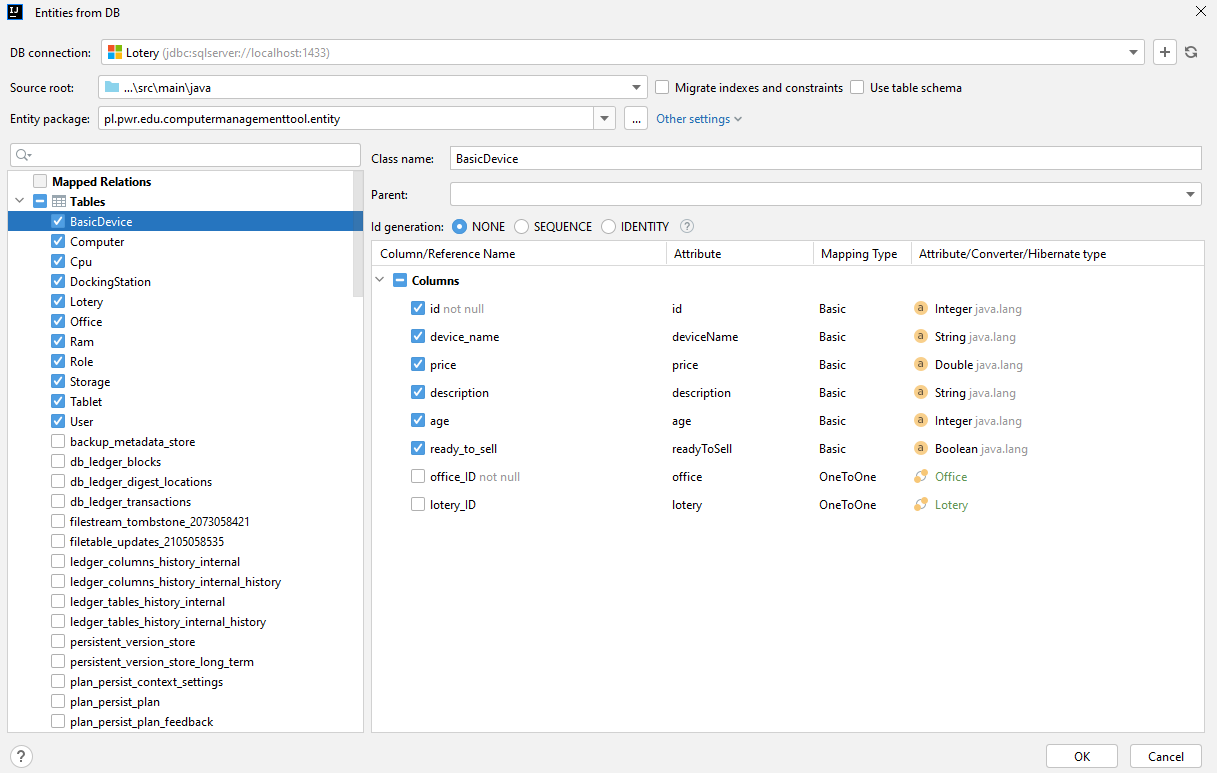
\includegraphics[scale=0.4]{rys05/generate_entities.png}
    \caption{Generowanie klas dla odpowiadających tabel}
    \label{entities_etykieta}
\end{figure}

JPA Buddy(odwolanie) pozwala na wygenerowanie klas odpowiadających tabelom w bazie danych Rys. \ref{entities_etykieta}

\newpage
\begin{figure}[h]
    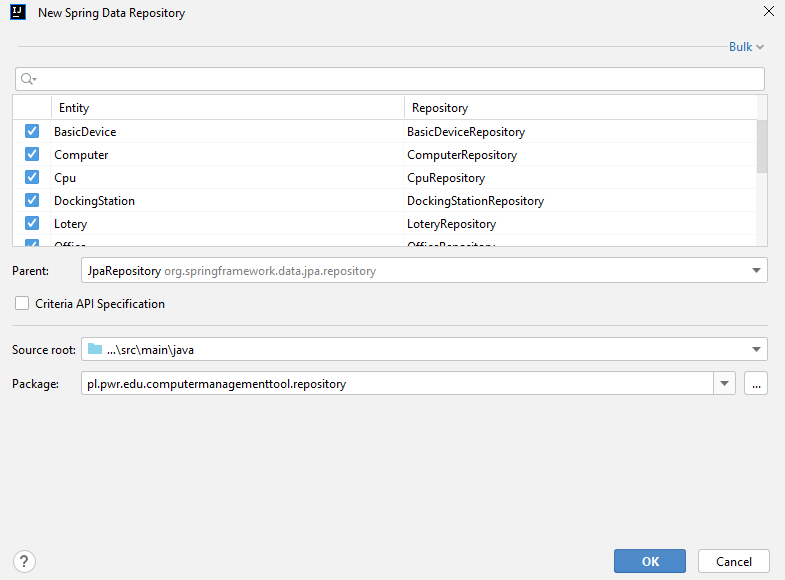
\includegraphics[scale=0.6]{rys05/generate_repository.png}
    \caption{Generowanie repozytorium dla odpowiadających tabel}
    \label{repository_etykieta}
\end{figure}

Pozwala też na wygenerowanie Repozytoriów Rys. \ref{repository_etykieta}. Pakiety klas takie jak Entiti, Service, Repository, Service opisano w rozdziale(nastepnym)


POPRZYCINAĆ ZDJĘCIA, TABLEA TECHNOLOGIE OPISAĆ, NASTEPNY ROZDZIAL STRUKTURA PROJEKTU, SPRINGBOOT


















